\section{Results}
\label{sec:results}

\subsection{Reference Performance in New Patients}
\label{sec:results:subtype_audit}

Table~\ref{tab:main} reports APT-only typing on the same 40 held-out patients.
Under the unified v2 protocol, fine SB-Macro-F1 is 0.134 for LR and XGBoost,
0.137 for MLP, 0.147 for Flat, 0.146 for HCE and 0.148 for Cascade without
disease supervision. The prespecified descriptive Flat-minus-MLP difference
is $+0.0100$ (paired 95\% CI $[-0.0047,0.0234]$), and Cascade-minus-Flat is
$+0.0011$ ($[-0.0093,0.0093]$). These intervals do not establish superiority
or equivalence. Models share input transforms, inner partitions and fresh
outer refits, but retain model-specific objectives and optimization budgets
(Appendix~\ref{sec:appendix:unified_v2}).

\begin{table}[H]
\centering\small
\setlength{\tabcolsep}{4pt}
\begin{tabular}{llcc}
\toprule
Model & CI & Fine SB-F1 $\uparrow$ & Coarse SB-F1 $\uparrow$ \\
\midrule
Logistic Regression & P & 0.134 [0.114, 0.146] & 0.296 [0.276, 0.315] \\
XGBoost & SP & 0.134 [0.118, 0.148] & 0.326 [0.304, 0.348] \\
Plain MLP & SP & 0.137 [0.121, 0.152] & 0.333 [0.307, 0.356] \\
Flat Transformer & SP & 0.147 [0.127, 0.162] & 0.342 [0.317, 0.365] \\
HCE Transformer & SP & 0.146 [0.126, 0.160] & 0.339 [0.316, 0.362] \\
Soft-cascade (no disease) & SP & 0.148 [0.129, 0.161] & 0.336 [0.311, 0.359] \\
\bottomrule
\end{tabular}
\caption{Unified v2 APT-only reference comparison on the same 361{,}792 OOF cells and 40 patients. All models use raw-count log1p inputs, training-only standardization, the same inner-patient split, and fresh refits on all 32 development patients. No main-table model uses disease supervision. Values are means across three training seeds (LR: one deterministic fit) with 5{,}000-resample pointwise 95\% intervals: P resamples patients; SP jointly resamples patients and seeds. LR/XGBoost select the two tasks separately; neural coarse scores are auxiliary outputs of fine-selected fits. HCE coarse scores use subtree probability mass. Model-specific search spaces and the selection-conditioned uncertainty target are given in Appendix~\ref{sec:appendix:unified_v2}.}
\label{tab:main}
\end{table}


\paragraph{Structure and extra supervision.}
Table~\ref{tab:unified_ablation} separates the full cascade structure from
cross-disease contrastive supervision. Adding contrastive supervision changes
fine SB-F1 by $+0.0006$ for Flat and $+0.0017$ for Cascade; their paired
intervals and the interaction interval include zero. This does not establish
that these recipes are equivalent or that hierarchy is unhelpful. In
particular, Cascade-minus-Flat changes the global/expert/routing combination,
not soft routing alone.
\begin{table}[t]
\centering\small
\setlength{\tabcolsep}{4pt}
\begin{tabular}{llcc}
\toprule
Recipe & Disease & Fine SB-F1 & Paired difference [95\% CI] \\
\midrule
A: Flat & No & 0.147 [0.127, 0.162] & --- \\
B: Flat & Yes & 0.148 [0.126, 0.163] & B$-$A: 0.0006 [-0.0057, 0.0071] \\
C: Cascade & No & 0.148 [0.129, 0.161] & C$-$A: 0.0011 [-0.0093, 0.0093] \\
D: Cascade & Yes & 0.150 [0.128, 0.166] & D$-$C: 0.0017 [-0.0087, 0.0123] \\
\bottomrule
\end{tabular}
\caption{Unified v2 $2\times2$ comparison of the whole cascade structure and cross-disease contrastive supervision. A and C reuse the main-table fits; B and D add the same contrastive term. Shared encoder, inputs and search rules are held fixed, but each recipe selects its own validation optimum. C$-$A is not a routing-only effect. The interaction (D$-$C)$-$(B$-$A) is 0.0012 [-0.0087, 0.0110]. Intervals are paired, pointwise and exploratory, not multiplicity-adjusted tests.}
\label{tab:unified_ablation}
\end{table}


\paragraph{Can predicted parents realize the oracle gain?}
Frozen-score diagnostics in Table~\ref{tab:unified_decoding} compare ordinary
subtype prediction with predicted-parent masking (D1), probability-consistent
combination (D2), and true-parent masking (D4). For the v2 MLP, fine SB-F1 is
0.137, 0.131, 0.134 and 0.376 respectively. Thus these two deployable readout
rules do not realize the oracle gain for this recipe. This is not a test of
all possible trained hierarchical classifiers. The prior-controlled analyses
below use their original, separately identified fits.

Five-lineage and 27-subtype tasks differ in cardinality, prevalence and label
boundaries. Their raw F1 difference alone does not identify an APT resolution
limit. The following prior-controlled comparisons instead ask what remains
recoverable within a known lineage. Full subtype reporting and the supporting
split-protocol comparison are retained in
Appendices~\ref{sec:appendix:subtype_audit} and
\ref{sec:appendix:protocol_sensitivity}.

\subsection{Within-Lineage Identity Is Recoverable, but Heterogeneous}
\label{sec:results:within_lineage}

True-lineage decoding masks each frozen fine score vector to the correct
parent's children. This is a privileged diagnostic, not a deployable prediction:
it supplies the reference parent at test time and narrows the candidate set.
We therefore compare it with training-only conditional priors and with a
stronger APT-only control that retrains after shuffling whole APT vectors within
each patient and true lineage. The shuffle preserves patient- and lineage-level
APT distributions while breaking each cell's original APT--subtype pairing.

Under the unified raw-count protocol, the MLP rises from 0.137 ordinary fine
SB-Macro-F1 to 0.376 with true-lineage decoding (Table~\ref{tab:apt_shuffle_signal}).
The corresponding patient-by-lineage-shuffled oracle is 0.216, giving a
real-minus-shuffled difference of $+0.160$ (95\% CI $[0.132,0.172]$);
the training-only conditional-proportion prior is 0.180. The Flat Transformer
replication gives a similar overall contrast, $+0.156$ ($[0.125,0.175]$).
Thus the oracle gain is not explained by candidate-set restriction or by the
preserved patient-by-lineage APT distribution alone. It supports cell-level
APT correspondence in this diagnostic setting, without identifying a molecular
mechanism or an assay information ceiling.

\begin{table}[t]
\centering\small
\setlength{\tabcolsep}{3pt}
\begin{tabular}{llcccc}
\toprule
Model & Scope & Real oracle & Shuffled oracle & Prior & Real $-$ shuffled \\
\midrule
MLP & All & 0.376 & 0.216 & 0.180 & \makecell{$+0.160$\\$[0.132,0.172]$} \\
Flat & All & 0.371 & 0.216 & 0.180 & \makecell{$+0.156$\\$[0.125,0.175]$} \\
\midrule
MLP & B & 0.469 & 0.182 & 0.193 & \makecell{$+0.288$\\$[0.229,0.321]$} \\
MLP & Myeloid & 0.265 & 0.111 & 0.124 & \makecell{$+0.155$\\$[0.125,0.182]$} \\
MLP & NK & 0.869 & 0.872 & 0.478 & \makecell{$-0.003$\\$[-0.011,0.004]$} \\
MLP & Other & 0.844 & 0.496 & 0.490 & \makecell{$+0.349$\\$[0.051,0.422]$} \\
MLP & T & 0.225 & 0.136 & 0.096 & \makecell{$+0.089$\\$[0.072,0.101]$} \\
\bottomrule
\end{tabular}
\caption{APT-only conditional-pairing diagnostic under true-lineage decoding
(fine SB-Macro-F1). Real APT keeps each cell's original APT vector; shuffled
APT retrains after permuting whole vectors within patient and true lineage in
each partition. The prior is the training-only conditional-proportion
expected-confusion baseline. MLP lineages are exploratory; Flat is the
prespecified overall replication. Intervals jointly resample patients,
training seeds and shuffle realizations. These privileged-label diagnostics
are not deployable scores.}
\label{tab:apt_shuffle_signal}
\end{table}


The signal is not uniform. For the MLP, the real-minus-shuffled oracle contrast
is positive for B, Myeloid, Other and T scopes, but unresolved and slightly
negative for NK ($-0.003$, $[-0.011,0.004]$), where real and shuffled oracle
scores are both high. This prevents a simple statement that every lineage
contains recoverable subtype information under APT. It instead shows that the
useful diagnostic signal depends on the parent lineage and its child taxonomy.

Error diagnostics explain why ordinary prediction remains difficult. Across
the v2 MLP, Flat, HCE and no-disease Cascade, roughly 73--74\% of ordinary
subtype errors cross parent lineages, and true-lineage decoding repairs about
64\% of those cross-parent errors. Even when the auxiliary coarse head predicts
the correct parent, the fine head still assigns an out-of-parent subtype for
14--18\% of such cells, showing imperfect coordination between the heads.
These are patient-balanced error rates, not additive components of Macro-F1.
Complete cross-model summaries and 27-by-27 ordinary/oracle matrices appear in
Appendix~\ref{sec:appendix:v2_failure_structure}.

Finally, a trained conditional subtype MLP asks whether this diagnostic signal
can be converted into deployable performance. The model uses a shared MLP
encoder, a lineage head, and within-lineage subtype heads trained only against
the true parent during training; at test time it predicts by
$q_{g(k)}(x)r_{k\mid g(k)}(x)$ without access to the true parent. Its ordinary
fine score is 0.138, compared with 0.137 for the ordinary v2 MLP
($+0.0008$, $[-0.0057,0.0056]$). Its true-lineage oracle score is 0.389,
but the deployable gain remains unresolved. The current evidence therefore
separates two statements: APT contains cell-level within-lineage signal under
the oracle diagnostic, and the simple conditional training recipe tested here
does not yet make that signal useful for overall deployed subtype prediction.

\paragraph{Does directly targeting the bottleneck help?}
We next keep the same MLP capacity and test fine-head parent-mass supervision,
coarse--fine consistency, privileged within-lineage distillation, and their
combinations (Table~\ref{tab:hbm_ablation}). A fresh reproduction of the v2 MLP
scores 0.136, close to the committed 0.137 reference. Distillation alone has
the largest new point estimate, 0.140; its paired difference from the reproduced
MLP is $+0.0040$ (95\% CI $[-0.0018,0.0087]$). Its overall cross-lineage error
does not fall ($+0.0011$, $[-0.0054,0.0068]$), and its oracle score rises more
than its ordinary score, so the hierarchy gap does not close. The full objective
scores 0.138 (difference $+0.0015$, $[-0.0025,0.0060]$) and changes cross-lineage
error by $+0.0045$ ($[-0.0005,0.0097]$). Its smaller oracle gap is driven mainly
by lower oracle performance (0.372 versus 0.378), not by the student approaching
the original oracle. Thus none of these objectives establishes a deployable
gain or reduces cross-lineage routing errors under the tested protocol.
\begin{table}[t]
\centering\small
\setlength{\tabcolsep}{3.2pt}
\resizebox{\linewidth}{!}{%
\begin{tabular}{lrrrrrr}
\toprule
Training objective & Fine & Coarse & Cross error & Outside $\mid$ coarse correct & Oracle & Gap \\
\midrule
Plain MLP & 0.136 & 0.335 & 0.491 & 0.176 & 0.378 & 0.242 \\
$+$ parent mass & 0.136 & 0.334 & 0.496 & 0.179 & 0.378 & 0.242 \\
$+$ parent mass $+$ consistency & 0.139 & 0.337 & 0.495 & 0.178 & 0.380 & 0.241 \\
$+$ distillation & \textbf{0.140} & 0.335 & 0.492 & 0.172 & 0.384 & 0.244 \\
$+$ parent mass $+$ distillation & 0.139 & 0.332 & 0.492 & 0.178 & 0.375 & 0.236 \\
Full HBM & 0.138 & 0.336 & 0.495 & 0.180 & 0.372 & 0.235 \\
\bottomrule
\end{tabular}}
\caption{Hierarchy-bottleneck mitigation with the unified MLP backbone.
Fine, coarse and oracle columns are subject-balanced Macro-F1; cross error is
the patient-balanced fraction of all predictions that are both wrong and
cross-lineage. Outside $\mid$ coarse correct is the fraction of cells whose
fine prediction leaves the true lineage among cells with a correct auxiliary
coarse prediction. Gap is oracle minus ordinary fine F1. Entries average three
matched seed slots over the same five patient folds. Oracle decoding supplies
the true lineage and is diagnostic, not deployable. Bold identifies the highest
deployable fine point estimate, not statistical superiority.}
\label{tab:hbm_ablation}
\end{table}


\begin{figure}[t]
\centering
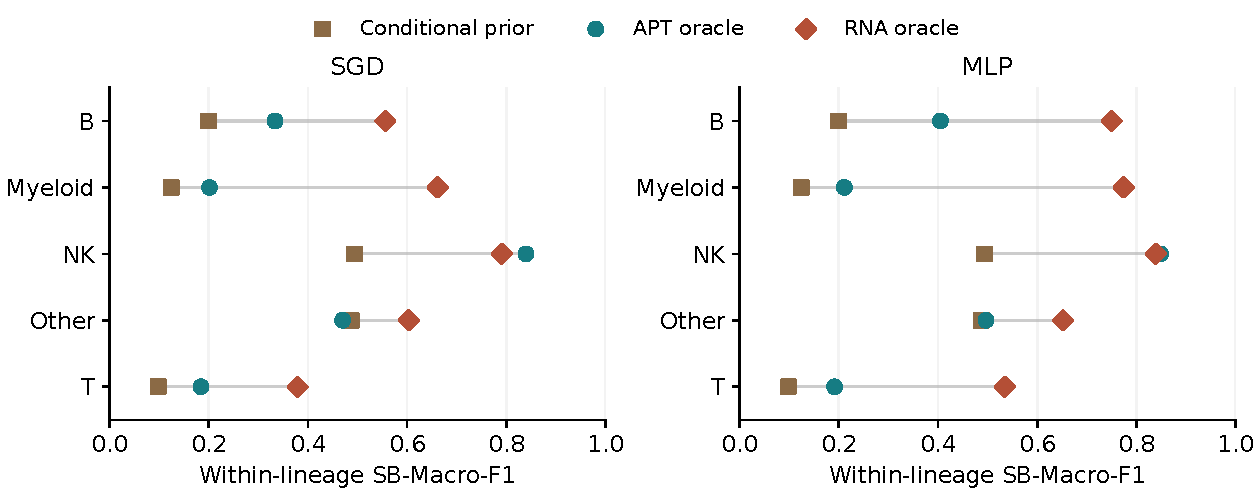
\includegraphics[width=\linewidth]{figures/matched_lineage_identity.pdf}
\caption{Matched-budget within-lineage reconstruction with 2,000
training-selected RNA HVGs. APT oracle, RNA oracle and conditional priors use
the same capped training subsets, patient folds and true-lineage information.
Points are means of three seed-specific scores, not F1 of seed-pooled
predictions; lines only connect methods within a lineage. Each patient's
matrix is normalized within the displayed lineage before pooling over
eligible patients and scoring its fixed children (38 patients for Other;
40 elsewhere). Consequently, these lineage scores cannot be averaged to
reconstruct the All row of Table~\ref{tab:matched_identity} from this same probe.
Row labels give the number of child subtypes.
These are descriptive point estimates, not superiority tests.
Expected-prior F1 is computed from an expected confusion matrix.}
\label{fig:matched_lineage_identity}
\end{figure}

The matched-input probe holds budget and recipe fixed across modalities
(Figure~\ref{fig:matched_lineage_identity}). MLP ordinary/oracle APT scores
are 0.093/0.309, RNA oracle is 0.672, and the expected prior is 0.182.
The APT oracle-minus-prior difference is $+0.127$ ($[0.101,0.139]$).
Relative to each lineage's own conditional prior and RNA reference,
APT reconstruction differs across lineages. Their absolute F1 values are
not a common biological-resolution scale: child-class counts and prevalence
also differ. For example, APT/RNA oracle scores are 0.849/0.839 for NK
but 0.191/0.535 for T cells. Knowledge of the parent therefore does not
uniformly resolve the RNA reconstruction gap. All lineages and both model
families are shown, without asserting an intrinsic modality ranking.

\paragraph{Budget and recipe matter.}
The full-budget MLP uses all development cells, a 256/128-unit network and
AdamW with selected stopping; the matched probe caps training at 1,000 cells
per patient and uses a 64-unit MLP for 40 epochs. Other has oracle F1 of
0.886 in the former but 0.497 in the latter (conditional expected priors
0.490/0.487). The recipes also differ in APT preprocessing
(Table~\ref{tab:identity_training_config}): log1p of raw counts in the matched
probe versus provided APT expression without an added log transform in the
full-budget MLP, each followed by training-set standardization.
Their score differences therefore cannot be attributed to training-cell budget alone.
Neither result justifies declaring Other universally identifiable or
unidentifiable. The full-budget lineage plot and neural-reference replays
are supporting evidence in Appendices~\ref{sec:appendix:full_budget_hierarchy}--\ref{sec:appendix:true_lineage_oracle}.

\subsection{Paired APT Improves on RNA, without Resolved Pairing Specificity}

Across three training seeds under the matched probe, MLP fine SB-Macro-F1 increases from 0.589 for RNA
to 0.607 for RNA+APT: $+\pairedMLPGainTwoK{}$ (joint 95\% CI $[0.009,0.030]$).
At 5,000 training-selected HVGs, it increases from 0.596 to 0.612:
$+\pairedMLPGainFiveK{}$ ($[0.009,0.029]$). SGD also improves at both widths
(Table~\ref{tab:paired_increment_main}). The increment is therefore not
specific to the 2,000-HVG setting, but remains relative to the tested RNA
representations and models.
Both widths use the capped-budget probe, not a full-cell-budget RNA model;
increasing HVGs does not control network capacity or training sufficiency.

\begin{table}[t]
\centering\small\setlength{\tabcolsep}{3pt}
\begin{tabular}{llcc}
\toprule
RNA HVGs & Comparator to paired RNA+APT & SGD $\Delta$ [95\% CI] & MLP $\Delta$ [95\% CI] \\
\midrule
2,000 & RNA & \makecell{$+0.0185$\\$[0.0034, 0.0332]$} & \makecell{$+0.0180$\\$[0.0092, 0.0297]$} \\
2,000 & RNA + noise & \makecell{$+0.0394$\\$[0.0240, 0.0537]$} & \makecell{$+0.0341$\\$[0.0208, 0.0448]$} \\
2,000 & Patient shuffle & \makecell{$+0.0059$\\$[-0.0049, 0.0165]$} & \makecell{$+0.0088$\\$[0.0014, 0.0145]$} \\
2,000 & Patient $\times$ lineage shuffle & \makecell{$+0.0064$\\$[-0.00437, 0.01657]$} & \makecell{$+0.0064$\\$[-0.00018, 0.01180]$} \\
\midrule
5,000 & RNA (width sensitivity) & \makecell{$+0.0217$\\$[0.0104, 0.0339]$} & \makecell{$+0.0165$\\$[0.0093, 0.0289]$} \\
\bottomrule
\end{tabular}
\caption{Overall fine SB-Macro-F1 differences, positive favoring paired
RNA+APT. Shuffle comparators append shuffled APT to RNA.
All 2,000-HVG contrasts use the same targeted experiment: three
training seeds and three realizations per seed for each shuffle type.
The 5,000-HVG row is the separate matched-width RNA comparison, not a
conditional-shuffle test. Scores are computed per fit before averaging;
2,000 paired seed/patient bootstrap replicates additionally resample shuffle
realizations where applicable. Intervals are pointwise and exploratory.
Both patient-by-lineage-shuffle intervals include zero.}
\label{tab:paired_increment_main}
\end{table}


\paragraph{What the controls establish.}
In the targeted 2,000-HVG experiment, MLP exceeds RNA+noise by 0.0341 and
patient-shuffled APT by 0.0088 (joint 95\% CI $[0.0014,0.0145]$).
This interval resamples patients, training seeds and shuffle realizations;
it is not a patient-only interval conditional on one fitted model.
The latter comparison uses three shuffle draws per
training seed, as does the more restrictive patient-by-lineage control.
Paired minus patient-by-lineage-shuffled APT is $+0.0064$
($[-0.00018,0.01180]$); SGD's corresponding interval also includes zero.
This is an unresolved overall contrast, not equivalence or evidence of no
pairing information. All control contrasts in the table come from the same
targeted experiment; the separate one-shuffle-per-seed width grid is labeled
as a sensitivity analysis in the appendix.
Lineage-specific contrasts remain exploratory supporting analyses
(Appendix~\ref{sec:appendix:identity_questions}).
